\chapter{Anwendung der Spieltheorie auf Vier Gewinnt}
\label{cha:nwendung der Spieltheorie auf Vier Gewinnt}
In diesem Kapitel werden die spieltheoretischen Aspekte von 4Gewinnt, einschließlich der Analyse von Spielsituationen, der Berechnung von Gewinnwahrscheinlichkeiten und der Entwicklung von Spielstrategien untersucht.


\section{Analyse von Spielsituationen}
\label{sec:Analyse von Spielsituationen}
Für das Verständnis der Spieldynamik und die Entwicklung effektiver Strategien, ist die Analyse der Spielsituation entscheidend.
Vier Gewinnt, ist ein zwei Personen Spiel mit vollständiger Information. Das bedeutet, alle Spieler zu jeder Zeit den gesamten Zustand des Spiels kennen \autocite{ruile2009viergewinnt}.

Der Bestimmungssatz von Ernst Zermelo besagt, dass sich jedes kombinatorische Spiel in eine der folgenden Kategorien einordnen lässt.
\begin{enumerate}
	\item  Der beginnende Spieler hat eine dominante Strategie. Wenn das Spiel optimal, ohne Fehler verläuft, gewinnt er die Partie.
	\item Der nachziehende Spieler 2 hat eine dominante Strategie. Wenn das Spiel optimal verläuft, gewinnt dieser.
	\item Keiner der beiden Parteien hat eine dominante Strategie. Wenn beide Spieler optimal spielen, endet das Spiel ohne einen Sieger. Sobald ein Spieler einen Fehler macht, gewinnt der andere Spieler das Spiel \autocite{mueller_2011}.
\end{enumerate}

Aus der Analyse geht hervor, dass bestimmte Situationen von besonderer Bedeutung für einen Sieg sind.
Das bilden einer horizontalen Viererreihe sind schwer zu erreichen. Umso wichtige ist es einen Sieg die Spalten 1-5 zu kontrollieren. 


\section{Berechnung von Gewinnwahrscheinlichkeiten}
Aufgrund der Komplexität des Spiels stellt die Berechnung der Gewinnwahrscheinlichkeit in Anwendung eine Herausforderung dar. Das Spielraster besteht aus sieben Spalten und sechs Zeilen, dadurch entsteht eine enorm große Anzahl an möglichen Zuständen. Was die Wahrscheinlichkeitsberechnung für den Gewinn des Spiels so komplex macht.
Moderne Ansätze zur Berechnung der Gewinnwahrscheinlichkeit greifen auf KI-Technik zurück. Die exakte Berechnung für alle möglichen Spielsituationen bleibt aufgrund der Komplexität von Vier Gewinnt eine Herausforderung \autocite{ruile2009viergewinnt}.
\section{Entwicklung von Spielstrategien}
	
Um eine spielstarke Strategie für 4Gewinnt mit dem Alpha-Beta-Algorithmus zu entwickeln und später zu programmieren, müssen mehrere Schritte beachtet werden. Hier wird der gesamte Prozess erläutert, von der Spielrepräsentation über die Bewertung von Stellungen bis hin zur Integration des Alpha-Beta-Algorithmus.

\subsection*{1. Spielfeld als Datenstruktur}
Zunächst muss das Spielfeld von 4Gewinnt in einer Form dargestellt werden, die von einem Algorithmus verarbeitet werden kann.
Hierzu kann ein 2D-Array (6 Zeilen × 7 Spalten) verwendet werden, das den Zustand des Spielfeldes beschreibt. Für jede Situation kann eine andere Zahl verwendet werden:
\begin{itemize}
	\item 0: Leeres Feld
	\item 1: Spielstein von Spieler 1
	\item -1: Spielstein von Spieler 2
\end{itemize}

Das Spielfeld kann nun als Array folgendermaßen dargestellt werden:

\[
\text{Spielfeld} =
\begin{pmatrix}
	0 & 0 & 0 & 0 & 0 & 0 & 0 \\
	0 & 0 & 0 & 0 & 0 & 0 & 0 \\
	0 & 0 & 0 & 0 & 0 & 0 & 0 \\
	0 & 0 & 0 & 0 & 0 & 0 & 0 \\
	0 & 0 & 0 & 0 & 0 & 0 & 0 \\
	0 & 0 & 0 & 0 & 0 & 0 & 0 \\
\end{pmatrix}
\]

\subsection*{2. Berechnung als Zugmöglichkeiten }
Da Spielsteine nur in den unteren freien Reihen platziert werden können, muss eine Funktion implementiert werden, die gültige Züge berechnet:

\begin{lstlisting}[language=Python, caption=Funktion zur Berechnung gültiger Züge]
	def gueltige_zuege(board):
	return [spalte for spalte in range(7) if brett[0][spalte] == 0]
\end{lstlisting}

\section*{3. Bewertung der Spielstellung}

Eine Bewertungsfunktion ist entscheidend für die Strategie. Sie schätzt den Wert einer Stellung ein und liefert eine Zahl:

\begin{itemize}
	\item \textbf{Gewinn für Spieler:} Sehr hoher Wert, z. B. \( +1000 \).
	\item \textbf{Verlust für Gegner:} Sehr niedriger Wert, z. B. \( -1000 \).
	\item \textbf{Potenzielle Verbindungen:} Punkte für 2er- und 3er-Reihen, die noch zu einem Sieg führen können.
	\item \textbf{Blockieren von Gegnerzügen:} Zusätzliche Punkte für Züge, die den Gegner daran hindern, 4 in eine Reihe zu bilden.
\end{itemize}

\section*{4. Alpha-Beta-Algorithmus implementieren}
	Der Alpha-Beta-Algorithmus wird verwendet, um den besten Zug zu berechnen, indem der Suchbaum effizient durchsucht wird. 
    Es geht darum, den besten Zug auszuwählen, basierend auf einer bestimmten Spielsituation und der Tiefe. Der Alpha-Beta-Algorithmus durchsucht den Entscheidungsbaum bis z.B. zur Tiefe 4 und nutzt alpha und beta, um unnötige Pfade auszulassen. maximizingPlayer=True gibt an, ob der Spieler seinen Vorteil maximiert.
\begin{lstlisting}[language=Python, caption=Alpha-Beta Algorithmus - Kurzer Überblick]
	# Alpha-Beta Algorithmus in Aktion
	bester_Zug = alpha_beta(board, Tiefe=4, alpha=-float('inf'), beta=float('inf'), maximizingPlayer=True)
	print(f"Bester Zug: Spalte {bester_Zug}")
\end{lstlisting}

\section*{5. Entscheidung für den besten Zug}

Im fünften Schritt geht es darum, den optimalen Zug für den aktuellen Spieler zu finden. Dazu werden alle möglichen Züge angeschaut und mithilfe dem Alpha-Beta-Algorithmus bewertet. Der Zug, der am besten abschneidet – je nachdem, ob der Spieler versucht, seinen Punktestand zu maximieren oder zu minimieren – wird dann ausgewählt. Dieser Schritt ist entscheidend für die Entscheidungsfindung und markiert das Ende der Analyse des Spielbaums.

\begin{lstlisting}[language=Python, caption=Entscheidung für den besten Zug - Überblick]
# Grober Aufbau der Funktion zur Zugentscheidung
def bester_zug(board, tiefe, spieler):
bester_wert = float('-inf') if spieler == 1 else float('inf')
beste_spalte = None

for spalte in gueltige_zuege(board):
zug_wert = alpha_beta(anwenden_zug(brett, spalte, spieler), tiefe - 1, -float('inf'), float('inf'), False)
if (spieler == 1 und zug_wert > bester_wert) or (spieler == -1 und zug_wert < bester_wert):
bester_wert = zug_wert
beste_spalte = spalte

return beste_spalte
\end{lstlisting}
\begin{itemize}

	\item Die Funktion \texttt{bester\_zug} ist darauf ausgelegt, den besten Zug für einen Spieler zu bestimmen. 
	\item \texttt{gueltige\_zuege(board)} gibt alle gültigen Spalten zurück, in die ein Stein gesetzt werden kann. 
	\item \texttt{anwenden\_zug(board, spalte, spieler)} simuliert das Setzen eines Steins in eine bestimmte Spalte. 
	\item Der \emph{alpha-beta}-Algorithmus wird auf das simulierte Spielfeld angewendet, um die Bewertung des Zugs zu berechnen. 
	\item Der Spieler wählt den Zug mit der höchsten Bewertung (für Maximierer) oder der niedrigsten Bewertung (für Minimierer).
\end{itemize}

\section*{5. Endzustände erkennen}

Für die Auswertung der Endzustände wird eine Funktion benötigt, um festzustellen, ob das Spiel vorbei ist. Es können zwei Endzustände eintreffen:
\begin{itemize}
	\item Einer der Spieler hat 4 Steine in einer Reihe.
	\item Das Spielfeld ist voll.
\end{itemize}

Die Funktion Endzustand\_erreicht überprüft, ob ein Endzustand in einem Spiel erreicht wurde, indem sie zwei Bedingungen prüft: ob ein Spieler gewonnen hat (über die Funktion Spieler\_gewinnt) oder ob das Spielfeld voll ist (über die Funktion Board\_voll). 

\begin{lstlisting}[language=Python, caption=Erkennung des Endzustands]
def Endzustand_erreicht(board):
return Spieler_gewinnt(board) or Board_voll(board[0][col] != 0 for col in range(7))
\end{lstlisting}

\section*{7. Spielstrategie optimieren}

Nach dem Programmieren der Spielstrategien steht die Optimierung im Vordergrund. Um die Effizienz zu steigern, sollten Suchtiefe und Zeitlimit angepasst werden.

Die \textbf{Suchtiefe} kann je nach \textbf{Rechenleistung} variiert werden, um ein gutes Gleichgewicht zwischen der Tiefe des Spielbaums und der benötigten Rechenzeit zu finden. Da der Algorithmus auf einem LEGO Spike Roboter läuft, ist die Rechenzeit begrenzt. Daher ist es sinnvoll, eine Tiefensuche zu implementieren, die es ermöglicht, innerhalb eines festgelegten Zeitlimits die bestmögliche Tiefe zu erreichen. 







\chapter{Systementwurf}

Es soll eine detaillierte und funktionsfähige Vorrichtung entworfen werden, die in der Lage ist, Spielsteine präzise und zuverlässig in die vorgesehenen Spalten des Spielständers einzuführen. Dazu muss der Mechanismus so gestaltet sein, dass er unterschiedliche Positionen des Spielständers ansteuern und die Spielsteine mit der nötigen Genauigkeit platzieren kann. Nach dem Einwurf des Spielsteins muss die Vorrichtung den Spielständer wieder für den nächsten Zug freigeben, was eine genaue Steuerung und Rückkehr in die Ausgangsposition erfordert. Die mechanische Konstruktion muss robust und wiederholgenau arbeiten, um einen flüssigen und störungsfreien Spielablauf zu gewährleisten.


\section{Komponenten}
Zur Verwendung stehen folgende Sensorik und Aktorik zur Verfügung:


\begin{itemize}
\item \textbf{großer LEGO® Technic Hub:}
Der Hub ist das Steuerungselement des Spike Prime Systems. Er umfasst sechs Ein-/Ausgänge, welche den Anschluss von Peripheriegeräten, wie Sensorik und Aktorik, ermöglicht. Mit einem Micro-USB-Anschluss und Bluetooth wird die Kommunikation mit kompatiblen Endgeräten hergestellt. Der Hub besitzt ein integriertes MicroPython-Betriebssystem mit einem 100-MHz-Prozessor. 
Weitere Ausstattungen sind:
Individuell anpassbaren Lichtmatrix (5x5)
Aufzeigen von wichtigen Informationen und Statusmeldungen
Tasten
Ermöglichen eine einfache Navigation und Steuerung durch Menüs 
Lautsprecher
6-achsigen Kreiselsensor

\begin{figure}[H]
	\centering
	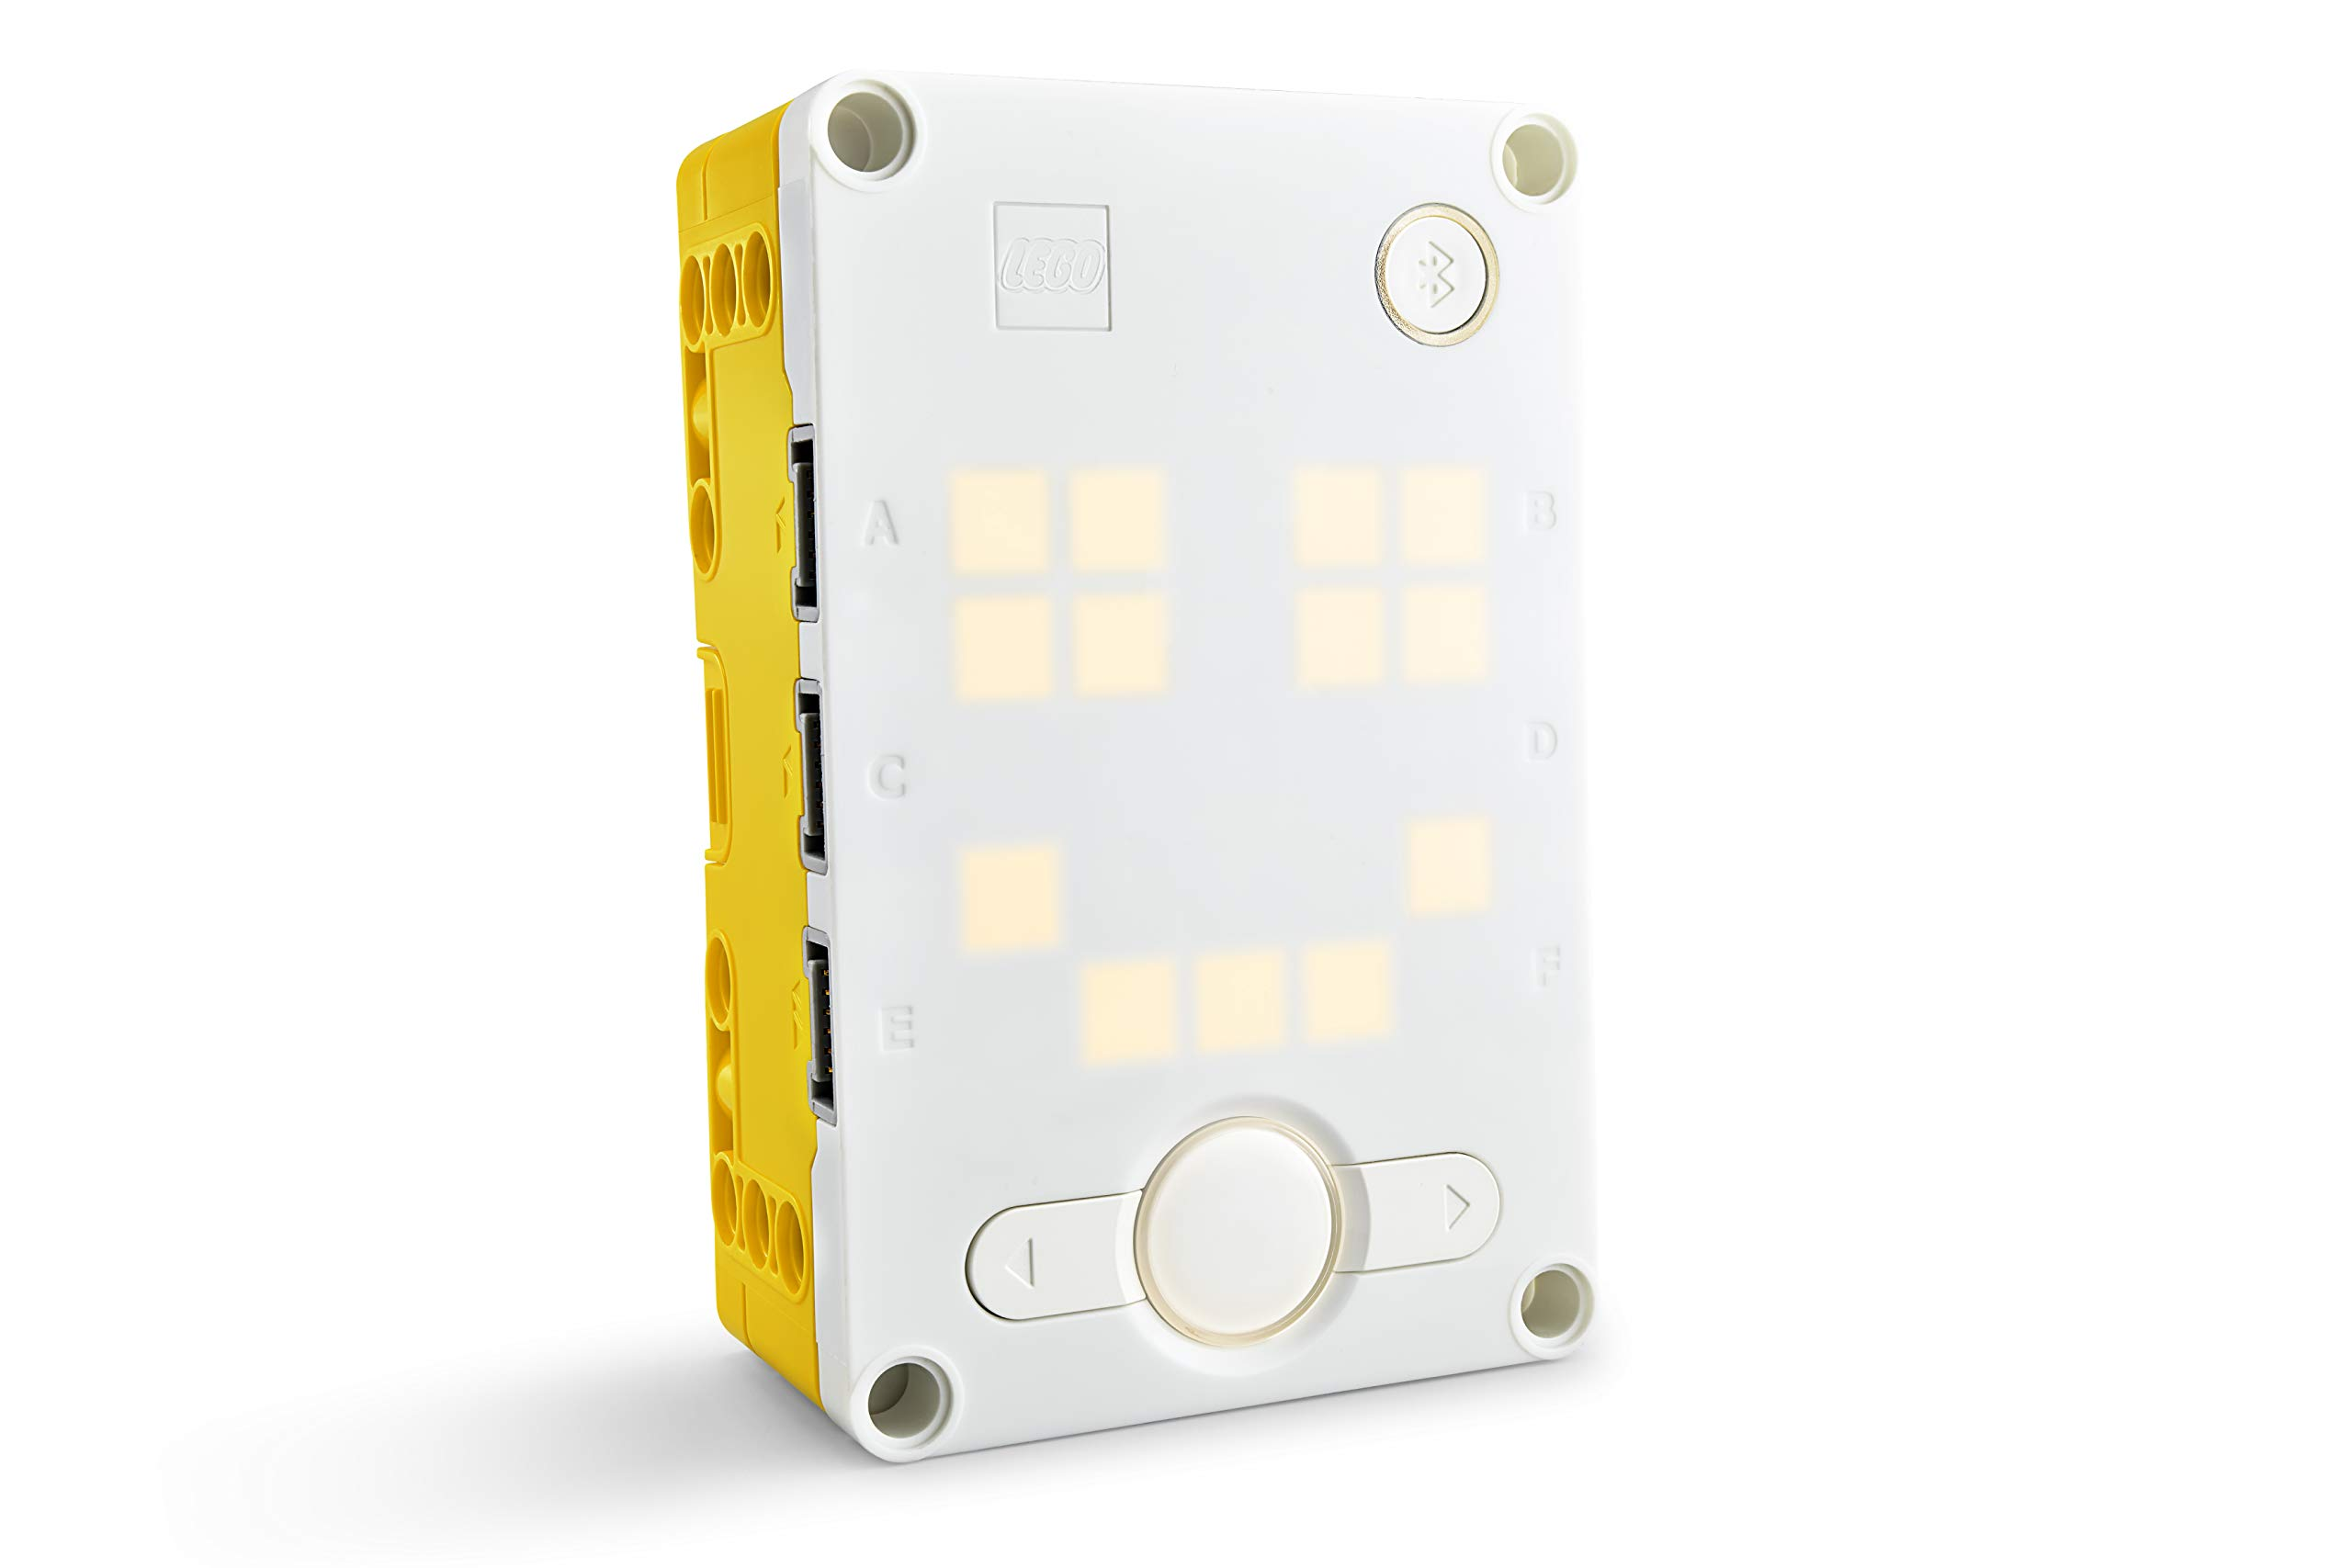
\includegraphics[width=0.5\linewidth]{images/Hub}
	\caption{Lego Technic Hub}
	\label{fig:hub}
\end{figure}


\item \textbf{LEGO® Technic Farbsensor:}
Dieser Sensor kann durch die Intensität des reflektierten Lichts, welche er durch den eingebauten Lichtring erzeugt, bis zu acht Farben erkennen und unterscheiden (erkennbare Farben: schwarz, blau, rot, weiß, braun, gelb, pink und grün).  Er wird vor allem bei Anwendungen, wie Sortieren nach Farben, Linienverfolgung von farbigen Streifen und zum Ausführen von farbcodierten Befehlen eingesetzt. Um die Farberkennung optimal auf die entsprechende Umgebung anzupassen, wird das Umgebungslicht zuvor ausgewertet.

\begin{figure}[H]
	\centering
	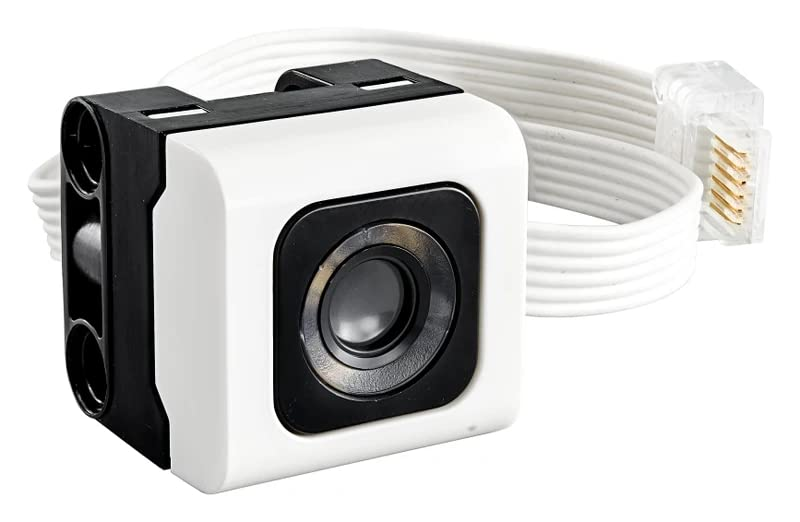
\includegraphics[width=0.5\linewidth]{images/Farbsensor}
	\caption{Lego Technic Farbsensor}
	\label{fig:farbsensor}
\end{figure}


\item \textbf{LEGO® Technic Großer Winkelmotor}
Für die Bewegungssteuerung wird dieser Winkelmotor mit hoher Drehkraft und präziser Steuerung verwendet. Dieser Motor ist dafür ausgelegt, um schwere und komplexe Konstruktionen exakt in Geschwindigkeit und Position verfahren zu können. Dies wird durch den internen Winkel- und Rotationssensor ermöglicht. Der Anwendungsbereich ist vielseitig, unter anderem wird dies als Antrieb von Rädern, Gelenke, Greifarme, Hebevorrichtungen und Drehscheibe angewandt. Vor allem für Aufgaben, welche eine genau und wiederholbare Aktion ausüben müssen.

\begin{figure}[H]
	\centering
	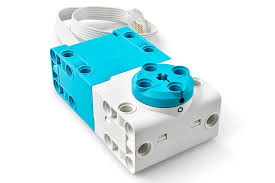
\includegraphics[width=0.5\linewidth]{images/Motor}
	\caption{Lego Technic Winkelmotor}
	\label{fig:motor}
\end{figure}

\end{itemize}

\section{Zusammenspiel von Soft- und Hardware}

Der LEGO SPIKE Farbsensor eignet sich hervorragend zur Erkennung der Spielsteine in einem Vier-Gewinnt-Spiel. 

\subsection{Mechanische Konstruktion des Farbsensor-Systems}

Das Farbsensor-System basiert auf einem zweiachsigen Antriebssystem, das eine präzise Bewegung sowohl in vertikaler als auch in horizontaler Richtung ermöglicht. 

Die \textbf{vertikale Bewegung} wird durch eine Kettenkonstruktion realisiert, an der der Farbsensor befestigt ist. Ein LEGO SPIKE Motor treibt die Kette präzise an und sorgt dafür, dass der Sensor alle sechs Reihen des Spielfeldes abtasten kann. 

Die \textbf{horizontale Bewegung} erfolgt über einen Wagen mit vier Rädern. Dieser Wagen wird durch einen zweiten Motor angetrieben, der mit Encoderwerten für eine präzise Positionierung gesteuert wird. Durch die horizontale Bewegung können alle sieben Spalten des Spielfeldes abgedeckt werden.

Die \textbf{Steuerung der Bewegungen} erfolgt durch eine koordinierte Ansteuerung beider Achsen, wodurch der Farbsensor schrittweise von Position zu Position bewegt wird. Optimierte Verfahrwege minimieren die Scanzeit, und eine Kalibrierung der Positionen gewährleistet eine genaue Ausrichtung des Sensors.

Diese mechanische Konstruktion ermöglicht eine zuverlässige und präzise Abtastung aller 42 Spielfeldpositionen des Vier-Gewinnt-Spiels und stellt somit eine optimale Grundlage für die Umsetzung  dar.
